\documentclass{beamer}
\usepackage{amsmath}


\begin{document}
\newcommand{\bmu}[1]{\underline{\boldsymbol{#1}}}

\begin{frame}
  \frametitle{Demand Equations and Parameters}
  Model parameters are in bold-underline; $\alpha_j$ is the budget
  fraction of component $j$.
    \begin{align}
    Q_s &=
    \bmu{A_s}\left(\frac{P_s}{P_m}\right)^{e_{ss}}\left(\frac{P_n}{P_m}\right)^{e_{sn}}\left(\frac{Y}{P_m}\right)^{h_s(Y)}.\\
    Q_n &=
    \bmu{A_n}\left(\frac{P_s}{P_m}\right)^{e_{ns}}\left(\frac{P_n}{P_m}\right)^{e_{nn}}\left(\frac{Y}{P_m}\right)^{h_n(Y)}.
    \end{align}
    where
    \begin{align}
      e_{ij} &= \bmu{g_{ij}} - \alpha_j
      \frac{\partial}{\partial \ln Y} \ln\left(\frac{Y}{P_m}\right)^{h_i(Y)}.\\
      h_s(Y) &= \bmu{\kappa}^{-\bmu{\lambda}}
      \left(\bmu{\kappa}Y\right)^{\bmu{\lambda}/Y}.\\
      h_n(Y) &= \frac{1}{2\bmu{\nu_1}}\left(Y\right)^{2\bmu{\nu_1}/\left(1-Y\right)}.
    \end{align}
\end{frame}

\begin{frame}
  \frametitle{Additional notes on Parameters}
  \begin{itemize}
    \item We require $g_{ij} = \frac{\alpha_j}{\alpha_i}g_{ji}$, so there are only three $g$
      parameters, which we label $g_{ss}$, $g_{nn}$, and
      $g_{\text{cross}}$.
    \item This makes a total of 8 parameters:
      \begin{itemize}
      \item 2 scale factors.
      \item 3 quasi-elasticities ($g$ matrix elements).
      \item 2 staple income dependence parameters.
      \item 1 nonstaple income dependence parameter.
      \end{itemize}
    \item The $\nu_1$ parameter is the income elasticity of nonstaple
      foods at $Y=1$, \emph{neglecting} the income dependence of the
      budget fractions, $\alpha$.
    \item The parameters in $h_s$ are not particularly intuitive, but
      they can be transformed to a more intuitive pair: $\mu_1$,
      $Y_0$.  These represent respectively the income elasticity at
      $Y=1$ (neglecting $\alpha$ dependence) and the income level at
      which elasticity switches from positive to negative.
  \end{itemize}
\end{frame}

\begin{frame}
  \frametitle{Likelihood Function and Monte Carlo}
  \begin{equation}
    L = \sum_i \frac{(y_i - \hat{y}_i)^2}{\sigma_i^2}
  \end{equation}
  For two sets of model parameters $\vec{p}_1$ and $\vec{p}_2$, the
  \emph{odds ratio} for the two parameter sets is
  \begin{equation}
    R_{12} = \exp\left(L_1 - L_2\right)
  \end{equation}
  So, a difference of 5 in $L$ indicates an odds ratio of about 150:1.
\end{frame}

\begin{frame}
  \frametitle{Monte Carlo Results (model v. 0.2)}
  \begin{center}
    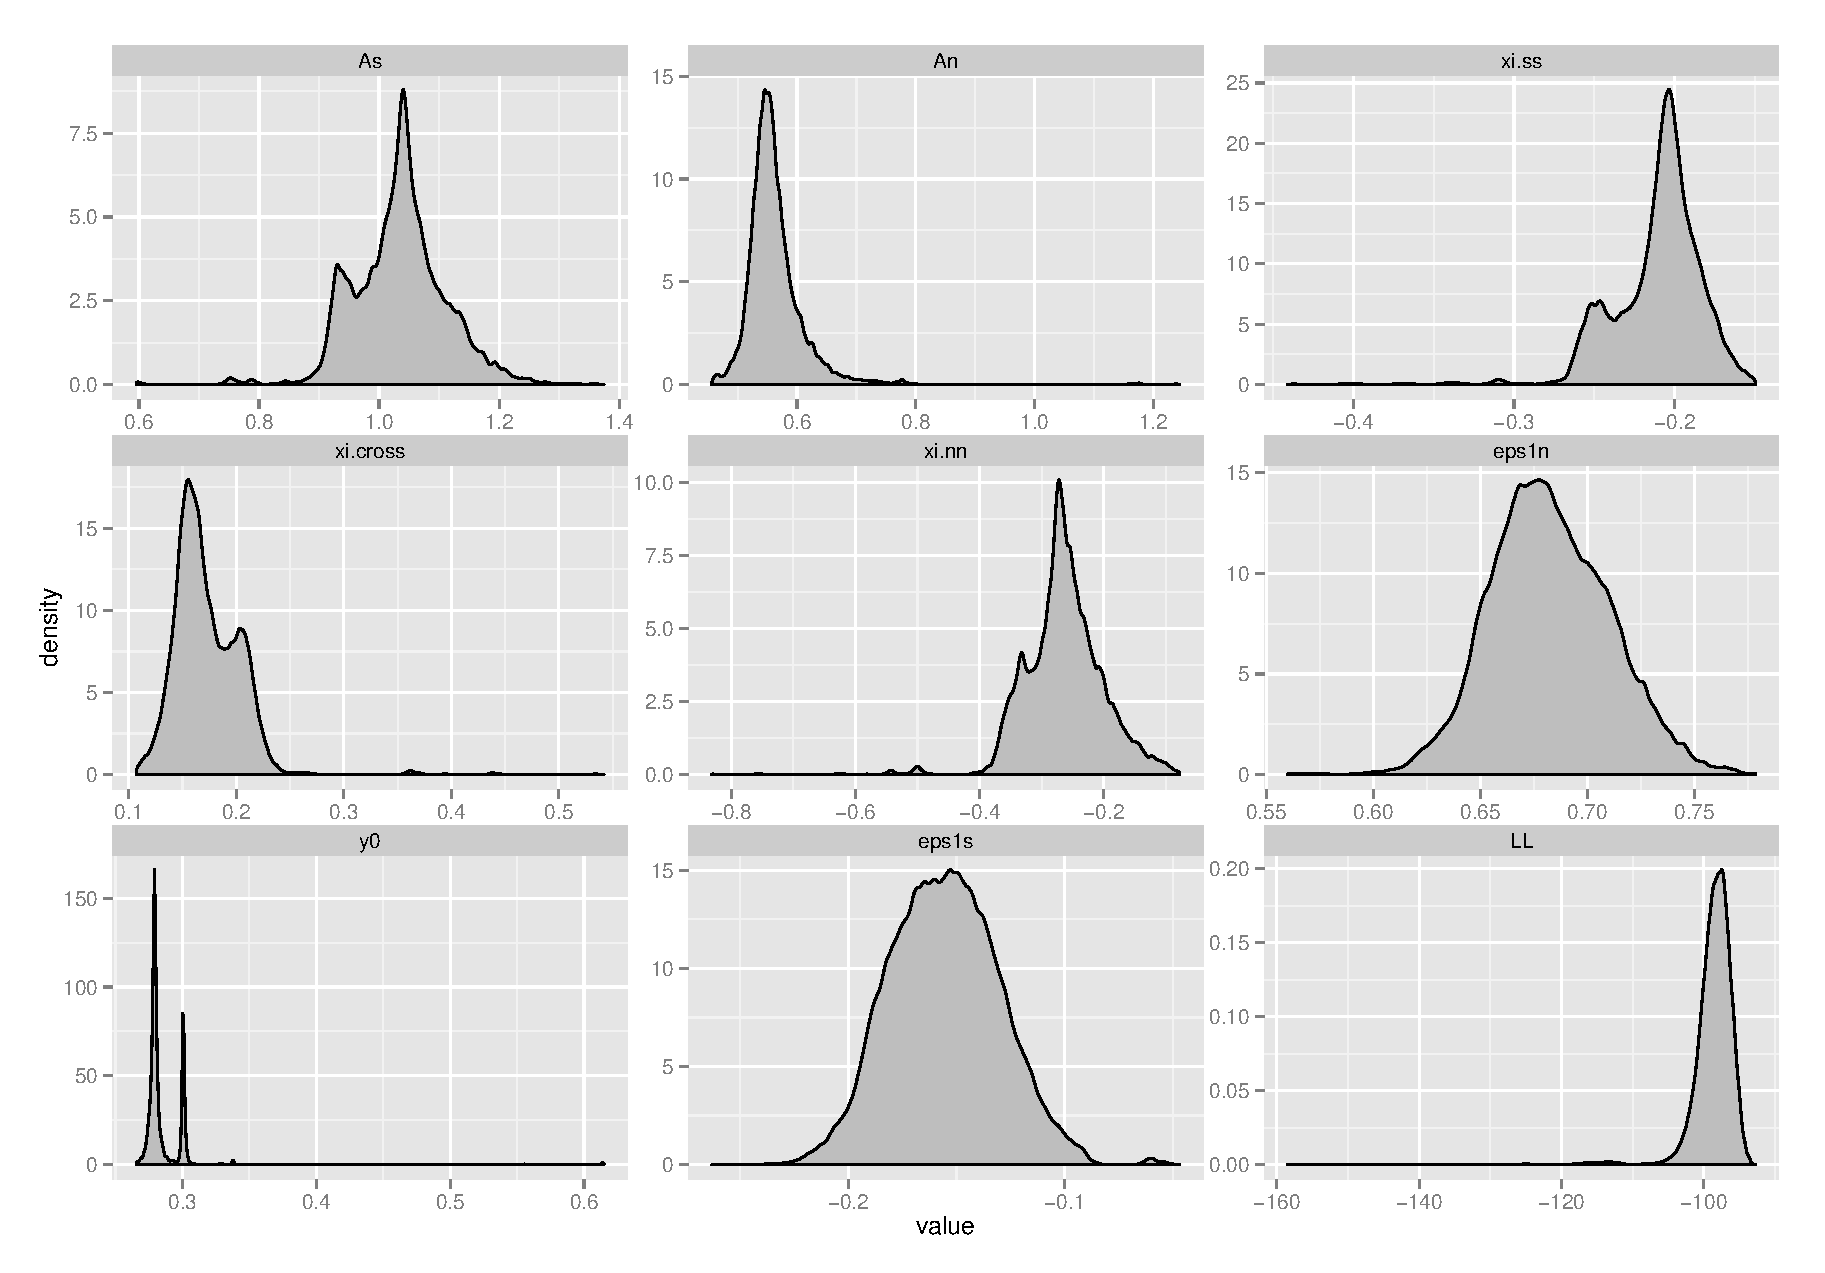
\includegraphics[width=0.85\textwidth]{fig/mcrslt-v0_2-allrgn.eps}
  \end{center}
\end{frame}

\end{document}
